\begin{table}[!htbp] \centering
	\label{tab:GSM1}
\begin{tabular}{|p{6cm}|p{8cm}|}
	\hline
		\textbf{Løsning}				&GSM Modul \\ \hline
		\textbf{Producent} 			&Cinterion \\ \hline
		\textbf{Interface} 			&I2C, SPI, USB \\ \hline
		\textbf{Beskrivelse} 		&Hardware modul der kan tilkobles X10'eren via SPI \\ \hline
		\textbf{Krav} 				&SIM kort og indgående programerings kendskab \\ \hline
		\textbf{Fordele}				&Mest pålidelige løsning og ingen forsinkelse på SMS'er \\ \hline
		\textbf{Ulemper} 			&Kræver viden inden for Java eller Microsoft Windows Mobile programering \\ \hline
		\textbf{Pris} 				&563,23 - 656,34 + SMS takst \\ \hline
		\textbf{Link} 				&http://dk.farnell.com/cinterion/mc75i/module-gsm-gprs-edge-quad-band/dp/1718875 \newline
									 http://dk.farnell.com/cinterion/tc65i/mod-gsm-gprs-quad-band-tcp-ip/dp/1718877 \\ \hline
		\multicolumn{2}{|c|}{
			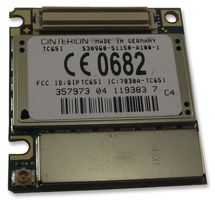
\includegraphics[height=3cm]{billeder/GSM_TC65I.jpg}} \\ \hline
\end{tabular}
\end{table}

\begin{table}[!htbp] \centering
	\label{tab:GSM2}
\begin{tabular}{|p{6cm}|p{8cm}|}
	\hline
		\textbf{Løsning}				&API \\ \hline
		\textbf{Producent} 			&Clickctell \\ \hline
		\textbf{Interface} 			&HTTP, HTTPS, FTP, SMPP, XML, SOAP, SMTP, COM obj.\\ \hline
		\textbf{Beskrivelse} 		&Software baseret API modul \\ \hline
		\textbf{Krav} 				&Forbindelse til internettet \\ \hline
		\textbf{Fordele}				&Let at programere \\ \hline
		\textbf{Ulemper} 			&Kræver forbindelse til internettet \\ \hline
		\textbf{Pris} 				&0,762 kr. pr. SMS \\ \hline
		\textbf{Link} 				&https://www.clickatell.com/apis-scripts/ \\ \hline	
		\multicolumn{2}{|c|}{
			
\includegraphics[height=3cm]{billeder/GSM_Clickatell.jpg}} \\ \hline	
\end{tabular}
\end{table}

\begin{table}[!htbp] \centering
	\label{tab:GSM3}
\begin{tabular}{|p{6cm}|p{8cm}|}
	\hline
		\textbf{Løsning}				&Arduino + GSM shield \\ \hline
		\textbf{Producent} 			&Arduino \\ \hline
		\textbf{Interface} 			&Internt \\ \hline
		\textbf{Beskrivelse} 		&Single-board computer med GSM modul\\ \hline
		\textbf{Krav} 				&SIM kort \\ \hline
		\textbf{Fordele}				&Let at programere \\ \hline
		\textbf{Ulemper} 			&\\ \hline
		\textbf{Pris} 				&149,- + 515,- + SMS takst\\ \hline
		\textbf{Link} 				&http://arduino.cc/ \\ \hline		
		\multicolumn{2}{|c|}{
			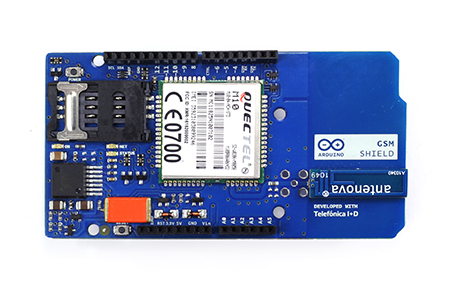
\includegraphics[height=3cm]{billeder/GSM_Arduino.jpg}} \\ \hline	
\end{tabular}
\end{table}

\subsection{Løsning}
Vi har valgt at bruge Clickatell løsning, da den er let at implementer, fleksibel og billig i opstarts omkostninger.